% !TEX program = pdflatex
% The Fixer Protocol: Side-Effect Tokenization for Decentralized Referral
% Incentives on Uniswap v4
% IEEE Conference Paper Format

\documentclass[conference]{IEEEtran}

% ============================================================================
% PACKAGES
% ============================================================================
\usepackage{cite}
\usepackage{amsmath,amssymb,amsfonts}
\usepackage{algorithmic}
\usepackage{graphicx}
\usepackage{textcomp}
\usepackage{xcolor}
\usepackage{hyperref}
\usepackage{booktabs}
\usepackage{multirow}
\usepackage{listings}
\usepackage{tabularx}
\usepackage{array}
\usepackage{url}
\usepackage{float}
\usepackage{caption}
\usepackage{subcaption}
\usepackage{tikz}
\usepackage{microtype}
\usetikzlibrary{shapes.geometric, arrows.meta, positioning, fit, calc}

% ============================================================================
% LISTINGS CONFIGURATION
% ============================================================================

% Define Solidity language for listings (must precede \lstset)
\lstdefinelanguage{Solidity}{
  keywords={function, returns, return, if, else, for, while, do, break, continue,
            contract, library, interface, struct, enum, mapping, address, uint256,
            uint128, uint64, uint8, int128, bool, bytes, bytes4, bytes32, string,
            memory, storage, calldata, external, internal, public, private, view,
            pure, payable, modifier, event, emit, require, revert, try, catch,
            this, super, true, false, immutable, constant, override, virtual,
            abstract, pragma, solidity, import, using, is, new, delete},
  sensitive=true,
  comment=[l]{//},
  morecomment=[s]{/*}{*/},
  string=[b]",
}

\lstset{
  language=Solidity,
  basicstyle=\ttfamily\footnotesize,
  keywordstyle=\color{blue}\bfseries,
  commentstyle=\color{gray},
  stringstyle=\color{red},
  breaklines=true,
  frame=single,
  captionpos=b,
  numbers=none,
  xleftmargin=2em,
  framexleftmargin=1.5em
}

% ============================================================================
% DOCUMENT
% ============================================================================
\begin{document}

\title{The Fixer Protocol: Side-Effect Tokenization for Decentralized Referral Incentives on Uniswap v4}

\author{\IEEEauthorblockN{Aaryan Guglani}
\IEEEauthorblockA{\textit{guglaniaaryan@gmail.com}\\
Atrium Academy (UHI8)\\
February 2026}}

\maketitle

% ============================================================================
% ABSTRACT
% ============================================================================
\begin{abstract}
Decentralized finance (DeFi) frontends, aggregators, and referrers drive the majority of swap volume on automated market makers (AMMs) yet receive no on-chain compensation for their contribution. Existing referral approaches either rely on centralized infrastructure or extract fees from swap participants, creating misaligned incentives. This paper presents the Fixer Protocol, an afterSwap hook for Uniswap v4 that introduces the Side-Effect Tokenization pattern---a mechanism by which referral reward tokens are minted as a pure side-effect of swap execution without modifying swap amounts or extracting fees from users. The protocol encodes referrer addresses in the hook data parameter and delegates to a UUPS-upgradeable registry that calculates volume-based rewards with tiered multipliers (1.0x--2.0x), applies protocol fees (5\%, capped at 10\%), and mints FIX tokens to the referrer. Safety mechanisms include circuit breakers (1M FIX/hour, 10M FIX/day), a 48-hour upgrade timelock, ERC-4337 Smart Account compatibility, soulbound NFT credentials (ERC-5192), and x402 agent support. Experimental evaluation demonstrates 314 passing tests across unit, fuzz, invariant, and integration categories, an average gas cost of 140,875 for referral processing, and successful deployment across three Layer-2 testnets. The Side-Effect Tokenization pattern establishes that hook-based reward systems can incentivize DeFi frontends without imposing any economic cost on users.
\end{abstract}

\begin{IEEEkeywords}
Uniswap v4, hooks, referral system, side-effect tokenization, DeFi incentives, UUPS proxy, soulbound NFT, smart contract security
\end{IEEEkeywords}

% ============================================================================
% I. INTRODUCTION
% ============================================================================
\section{Introduction}
\label{sec:intro}

The decentralized finance ecosystem has experienced sustained growth in automated market maker (AMM) protocols, with Uniswap alone facilitating over \$2 trillion in cumulative trading volume~\cite{uniswapv4}. Despite this growth, a fundamental misalignment persists between the entities that generate swap volume and those that capture value from it. Frontends, aggregators, and referrers---collectively responsible for directing the vast majority of user traffic to liquidity pools---receive no on-chain compensation for their contribution~\cite{frontendproblem}. This creates a free-rider problem where frontend operators must rely on off-chain business models, venture capital subsidies, or unsustainable fee extraction to remain operational.

Traditional referral programs in centralized exchanges and Web2 platforms rely on centralized databases, off-chain tracking, and manual settlement. These approaches are incompatible with the trustless, permissionless ethos of DeFi. Prior attempts at on-chain referral systems have typically involved fee extraction from swap participants, which degrades user experience and creates a misalignment between referrer incentives and user outcomes~\cite{flashboys}.

The introduction of Uniswap v4's hook architecture~\cite{uniswapv4} creates a new paradigm for extending AMM functionality. Hooks are external smart contracts that the PoolManager invokes at specific points in the pool lifecycle, including before and after swaps, liquidity modifications, and donations. Crucially, hooks can observe swap execution without modifying the core swap logic, enabling a new class of \textit{observation-only} extensions that enrich the swap lifecycle without altering its economics.

This paper presents the Fixer Protocol, which exploits this observation-only capability to implement on-chain referral rewards through a novel \textit{Side-Effect Tokenization} pattern. The protocol mints reward tokens as a pure side-effect of swap execution---the swap itself remains completely unmodified, and the user receives exactly the tokens they would without the hook. The referrer, encoded in the swap's \texttt{hookData} parameter, receives FIX tokens as compensation for directing the swap to the pool.

The contributions of this paper are:

\begin{enumerate}
    \item \textbf{Side-Effect Tokenization Pattern}: A novel design pattern for Uniswap v4 hooks where reward tokens are minted as a side-effect of swap observation, without extracting fees or modifying swap amounts (Section~\ref{sec:design}).

    \item \textbf{Tiered Referrer System}: A four-tier reward multiplier system (Bronze 1.0x, Silver 1.25x, Gold 1.5x, Platinum 2.0x) with automatic promotion based on cumulative volume and referral count (Section~\ref{sec:impl:tier}).

    \item \textbf{Production-Grade Architecture}: A UUPS-upgradeable smart contract system with ERC-7201 namespaced storage, circuit breakers, 48-hour upgrade timelock, soulbound NFT credentials, and ERC-4337 compatibility (Sections~\ref{sec:impl:fee}--\ref{sec:impl:x402}).

    \item \textbf{Comprehensive Experimental Validation}: 314 passing tests (55 unit, 31 fuzz, 4 invariant, 224 integration) with gas benchmarking and deployment verification on three Layer-2 testnets (Section~\ref{sec:eval}).
\end{enumerate}

The remainder of this paper is organized as follows. Section~\ref{sec:background} provides background on Uniswap v4 and related work. Section~\ref{sec:design} describes the system design and \textit{Side-Effect Tokenization} pattern. Section~\ref{sec:impl} details the implementation. Section~\ref{sec:eval} presents experimental results. Section~\ref{sec:security} analyzes security. Section~\ref{sec:discussion} discusses limitations and future work. Section~\ref{sec:conclusion} concludes.

% ============================================================================
% II. BACKGROUND AND RELATED WORK
% ============================================================================
\section{Background and Related Work}
\label{sec:background}

\subsection{Uniswap v4 Architecture}

Uniswap v4~\cite{uniswapv4} represents a fundamental architectural departure from its predecessors~\cite{uniswapv2,uniswapv3}. The protocol introduces a \textit{singleton} architecture where all pools reside within a single PoolManager contract, eliminating separate factory-deployed pool contracts. This singleton design reduces gas costs by enabling flash accounting, where token transfers are deferred and netted across multiple operations within a single transaction.

The most significant innovation in Uniswap v4 is the \textit{hooks} system. Hooks are external smart contracts that the PoolManager invokes at specific lifecycle points. The protocol defines 14 hook callbacks organized into seven \texttt{before}/\texttt{after} pairs covering five lifecycle events (\texttt{Initialize}, \texttt{Add\-Liquidity}, \texttt{Remove\-Liquidity}, \texttt{Swap}, \texttt{Donate}) and four return-delta variants that enable hooks to modify token balances.

Hook permissions are encoded directly in the hook contract's address through specific bit flags. The PoolManager inspects these bits to determine which callbacks to invoke, eliminating the need for on-chain permission registries. This design imposes a CREATE2 address-mining requirement during deployment, where the deployer must find a salt that produces an address with the correct permission bits set.

\subsection{Hook Permission Model}

Each hook callback corresponds to a specific bit in the hook contract's address. The Fixer Protocol enables only the \texttt{afterSwap} callback (bit 7), resulting in a minimal permission surface. This is a deliberate design choice: by avoiding \texttt{beforeSwap}, the hook cannot front-run or manipulate the swap, and by avoiding return-delta variants (\texttt{after\-Swap\-Return\-Delta}), the hook cannot modify the tokens received by the user.

The permission model is expressed in the \texttt{getHookPermissions()} function, which returns a \texttt{Hooks.Permissions} struct with only \texttt{afterSwap: true} and all other 13 fields set to \texttt{false}.

\subsection{Related Work}

\textbf{MEV Redistribution.} Flashbots~\cite{flashbots} and related projects have explored mechanisms for redistributing Maximal Extractable Value (MEV) to users or protocols. While MEV redistribution addresses value leakage at the block-production level, it does not solve the frontend incentivization problem at the application level. The Fixer Protocol operates orthogonally to MEV redistribution, as its rewards are volume-based rather than MEV-derived.

\textbf{Frontend Fee Systems.} Several DeFi protocols have experimented with explicit frontend fees, where frontends add a surcharge to swap transactions. These approaches create a direct cost to users and suffer from competitive pressure---users migrate to frontends that charge lower or no fees. In contrast, the \textit{Side-Effect Tokenization} pattern imposes no cost on users, as the reward token is newly minted rather than extracted from swap proceeds.

\textbf{Loyalty and Referral Tokens.} Centralized exchanges have deployed referral programs that offer fee rebates or native token rewards. These systems rely on centralized infrastructure for tracking and settlement~\cite{flashboys}. On-chain loyalty programs demonstrate the potential for token-based incentive mechanisms but operate in fundamentally different market structures.

\textbf{Soulbound Tokens.} Buterin~\cite{soulbound} introduced the concept of soulbound tokens (SBTs) as non-transferable credentials representing commitments, affiliations, or achievements. The Fixer Protocol extends this concept through FixerCredential, an ERC-5192-compliant~\cite{erc5192} soulbound NFT serving as an on-chain reputation credential for referrers. Unlike application-level badges stored off-chain, these credentials maintain integrity independent of any particular frontend or indexing service.

\textbf{Upgradeable Proxy Patterns.} OpenZeppelin's UUPS pattern~\cite{openzeppelin} enables smart contract upgradeability while maintaining a stable address. The Fixer Protocol augments the standard UUPS pattern with a 48-hour timelock to provide users with an exit window before upgrades take effect, addressing a common criticism of upgradeable contracts in DeFi.

\textbf{ERC-7201 Namespaced Storage.} Traditional upgradeable contracts store state variables sequentially, making storage layout changes across upgrades error-prone. ERC-7201~\cite{erc7201} introduces deterministic storage namespaces where the storage slot is derived from a human-readable namespace string. This eliminates slot collision risks and enables modular storage composition.

The system additionally builds upon ERC-20~\cite{erc20}, ERC-721~\cite{erc721}, ERC-4906~\cite{erc4906}, EIP-3009~\cite{eip3009}, ERC-4337~\cite{erc4337}, and ERC-1967~\cite{erc1967}.

\textbf{Reactive Network.} Reactive Network~\cite{reactivenetwork} is a relay chain that enables reactive smart contracts (RSCs)---contracts that autonomously subscribe to on-chain events from multiple origin chains and execute callback logic in response. Unlike bridge-based approaches that require explicit cross-chain message passing, RSCs use an event-driven model where a contract on the Reactive Network's ReactVM monitors \texttt{LogEmitted} events from specified origin chains and triggers destination-chain transactions without manual intervention. The Fixer Protocol's design doc identifies Reactive Network as the planned cross-chain layer for aggregating referral statistics across deployments on Base, Arbitrum, Unichain, and Ethereum. A Reactive Callback Proxy (\texttt{0xa6eA...5a6}) has been provisioned on Base Sepolia for the Lasna testnet (chain ID 5318007) integration.

\textbf{Hook-Based Protocol Extensions.} The emerging ecosystem of Uniswap v4 hooks has produced diverse extensions including dynamic fee adjusters, oracle integrations, and limit order systems. However, referral incentivization hooks remain underexplored. The Fixer Protocol contributes to this space by demonstrating that observation-only hooks can create value through side-effect mechanisms without interfering with core AMM functionality.

% ============================================================================
% III. SYSTEM DESIGN AND ARCHITECTURE
% ============================================================================
\section{System Design and Architecture}
\label{sec:design}

\subsection{The Side-Effect Tokenization Pattern}

The core design principle of the Fixer Protocol is \textit{Side-Effect Tokenization}---the minting of reward tokens as a side-effect of swap observation rather than through fee extraction or swap modification. This pattern is enabled by Uniswap v4's hook architecture, which allows the \texttt{afterSwap} callback to execute arbitrary logic after the swap has been completed and the pool state has been updated.

The key property of this pattern is that the \texttt{afterSwap} callback returns \texttt{(this.afterSwap.selector,\allowbreak{} int128(0))}, where the second value explicitly indicates zero delta modification. The swap proceeds identically to how it would without the hook---the user receives the exact same tokens at the exact same price. The reward to the referrer is a newly minted token (FIX) that exists independently of the swap's token pair.

This design eliminates the fundamental tension present in fee-extraction models, where the referrer's incentive (maximize fees) is misaligned with the user's interest (minimize fees). Under \textit{Side-Effect Tokenization}, both parties benefit: the user receives an unmodified swap, and the referrer receives a reward proportional to the volume they facilitated.

\subsection{Referral Encoding}

Referrer information is transmitted through the \texttt{hookData} parameter of the swap function. The frontend encodes the referrer's Ethereum address using standard ABI encoding:

\begin{lstlisting}[language=Solidity]
bytes memory hookData = abi.encode(referrerAddress);
\end{lstlisting}

The hook decodes this data in the \texttt{afterSwap} callback using a try/catch pattern to handle malformed data gracefully:

\begin{lstlisting}[language=Solidity]
try this.decodeReferrer(hookData)
    returns (address decoded) {
    referrer = decoded;
} catch {
    // Malformed data - skip silently
    return (this.afterSwap.selector, 0);
}
\end{lstlisting}

This encoding approach is minimally invasive: frontends that wish to participate simply include the referrer address in \texttt{hookData}, while frontends that do not participate pass empty \texttt{hookData}, which the hook handles with an early return.

\subsection{Architectural Evolution}

The protocol has evolved through three major architectural iterations:

\textbf{Version 1 (Monolithic).} The initial implementation combined the hook, reward token, and all business logic in a single contract (\texttt{FixerHook}, 755 lines). This contract employed a dual inheritance pattern, extending both \texttt{BaseHook} (from Uniswap v4-periphery) and \texttt{ERC20} (from Solady). While simple to deploy, this design coupled the hook's lifecycle to the token's lifecycle and prevented cross-pool reward aggregation.

\textbf{Version 2 (Modular).} The second iteration separated concerns into a lightweight hook (\texttt{FixerHookV2}, 361 lines) and a central registry (\texttt{FixerRegistry}). The hook performs only validation and volume calculation, then delegates referral recording to the registry via \texttt{recordReferral()}. This separation enables multiple hooks (one per pool) to share a single registry, enabling cross-pool referral tracking.

\textbf{Version 2.2+ (Upgradeable).} The current production architecture~\cite{fixerdesign} introduces UUPS upgradeability (\texttt{Fixer\-Registry\-Upgradeable}, 1,062 lines) with ERC-7201 namespaced storage~\cite{erc7201}, a 48-hour upgrade timelock, circuit breakers, and protocol fee distribution. This version adds the \texttt{FixerCredential} soulbound NFT and x402 agent support.

\subsection{Swap Flow}

The complete swap flow with referral processing is depicted in Fig.~\ref{fig:swapflow}. The key observation is that the swap amounts returned to the user are unmodified---the \texttt{afterSwap} hook returns \texttt{int128(0)}, indicating zero modification to the swap delta. All reward processing occurs as a side-effect.

\begin{figure}[t]
\centering
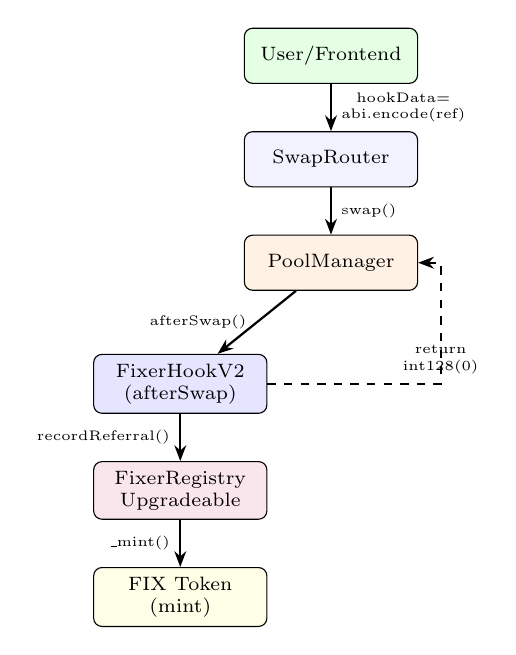
\begin{tikzpicture}[
    node distance=0.6cm,
    box/.style={rectangle, draw, rounded corners=3pt, minimum width=2.2cm, minimum height=0.7cm, font=\scriptsize, align=center, fill=blue!5},
    arrow/.style={-{Stealth[length=2mm]}, thick},
    label/.style={font=\tiny, align=center}
]
\node[box, fill=green!10] (user) {User/Frontend};
\node[box, below=of user] (router) {SwapRouter};
\node[box, below=of router, fill=orange!10] (pm) {PoolManager};
\node[box, below left=0.8cm and -0.3cm of pm, fill=blue!10] (hook) {FixerHookV2\\(afterSwap)};
\node[box, below=of hook, fill=purple!10] (reg) {FixerRegistry\\Upgradeable};
\node[box, below=of reg, fill=yellow!10] (fix) {FIX Token\\(mint)};

\draw[arrow] (user) -- node[right, label] {hookData=\\abi.encode(ref)} (router);
\draw[arrow] (router) -- node[right, label] {swap()} (pm);
\draw[arrow] (pm) -- node[left, label] {afterSwap()} (hook);
\draw[arrow] (hook) -- node[left, label] {recordReferral()} (reg);
\draw[arrow] (reg) -- node[left, label] {\_mint()} (fix);
\draw[arrow, dashed] (hook.east) -- ++(2.2,0) node[above, label] {return\\int128(0)} |- (pm.east);
\end{tikzpicture}
\caption{Swap flow with Side-Effect Tokenization. The \texttt{afterSwap} hook processes referral rewards entirely as a side-effect; swap amounts returned to the user are unmodified (\texttt{int128(0)}).}
\label{fig:swapflow}
\end{figure}

\subsection{Trusted Router Pattern}

In Uniswap v4, the \texttt{sender} parameter in hook callbacks refers to the router contract, not the end user. Identifying the actual user who initiated the swap is necessary for self-referral prevention. The protocol implements the Trusted Router Pattern to resolve the actual swapper:

\begin{enumerate}
    \item If the sender is a trusted router (maintained via an allowlist), the hook calls \texttt{IMsgSender(sender).\allowbreak{}msgSender()} to retrieve the authenticated end user.
    \item If the call fails or the sender is not trusted, the hook falls back to \texttt{tx.origin}.
\end{enumerate}

This pattern is compatible with ERC-4337 Smart Accounts~\cite{erc4337}, where \texttt{tx.origin} would be a bundler rather than the actual user.

% ============================================================================
% IV. IMPLEMENTATION
% ============================================================================
\section{Implementation}
\label{sec:impl}

\subsection{Contract Architecture}

The production deployment consists of four primary contracts and supporting libraries:

\textbf{FixerHookV2} (361 lines) serves as the lightweight, per-pool hook. It stores immutable references to the registry, pool ID, and quote token index. The contract contains no token logic and minimal storage (only the \texttt{trustedRouters} mapping), delegating all reward processing to the registry.

\textbf{FixerRegistryUpgradeable} (1,062 lines) is the central registry deployed behind an ERC-1967 proxy~\cite{erc1967}. This contract inherits from six OpenZeppelin upgradeable modules: \texttt{Initializable}, \texttt{UUPS\-Upgradeable}, \texttt{Ownable\-Upgradeable}, \texttt{ERC20\-Upgradeable}, \texttt{Reentrancy\-Guard\-Upgradeable}, and \texttt{EIP712\-Upgradeable}, plus the custom \texttt{Emergency\-Module} and \texttt{IAgent\-Registry} interface.

\textbf{FixerCredential} (397 lines) is a soulbound NFT credential contract implementing ERC-721~\cite{erc721} (via Solmate~\cite{solmate}), ERC-5192~\cite{erc5192} (soulbound semantics), and ERC-4906~\cite{erc4906} (metadata update events). It generates on-chain SVG artwork with tier-specific colors and fetches live stats from the registry for metadata rendering.

\textbf{FixerRegistryStorage} (266 lines) implements ERC-7201~\cite{erc7201} namespaced storage. All state variables are stored in a single \texttt{MainStorage} struct at a deterministic storage slot computed as:

\begin{small}
\noindent\texttt{keccak256(abi.encode(uint256(}\\
\texttt{\ \ keccak256("fixer.registry.storage}\\
\texttt{\ \ .main")) - 1))}\\
\texttt{\ \ \& \textasciitilde bytes32(uint256(0xff))}
\end{small}

\textbf{BPSMath} (47 lines) provides centralized basis-point arithmetic using Solady's~\cite{solady} \texttt{Fixed\-Point\-Math\-Lib.mul\-Div} for overflow-safe computation.

\subsection{Tier System}
\label{sec:impl:tier}

The protocol implements a four-tier referrer system where each tier provides an increasing reward multiplier. Tier promotion is automatic and occurs within the same transaction that triggers the threshold crossing. The tier thresholds, verified on-chain from the Base Sepolia deployment via \texttt{cast call}, are presented in Table~\ref{tab:tiers}.

\begin{table}[t]
\caption{Referrer Tier Thresholds (Verified On-Chain)}
\label{tab:tiers}
\centering
\begin{tabular}{lrrrc}
\toprule
\textbf{Tier} & \textbf{Min Vol.\ (USD)} & \textbf{Min Refs} & \textbf{Mult.} & \textbf{BPS} \\
\midrule
Bronze & 0 & 0 & 1.00x & 10,000 \\
Silver & 10,000 & 10 & 1.25x & 12,500 \\
Gold & 100,000 & 50 & 1.50x & 15,000 \\
Platinum & 1,000,000 & 200 & 2.00x & 20,000 \\
\bottomrule
\end{tabular}
\end{table}

The reward for a given swap is computed as:
\begin{align}
r_{\text{base}} &= V \cdot \frac{r_{\text{bps}}}{10{,}000} \label{eq:base-reward} \\
r_{\text{tier}} &= r_{\text{base}} \cdot \frac{m_{\text{bps}}}{10{,}000} \label{eq:tier-reward} \\
r_{\text{agent}} &= r_{\text{tier}} \cdot \frac{a_{\text{bps}}}{10{,}000} \quad \text{(if verified)} \label{eq:agent-reward} \\
r_{\text{gross}} &= r_{\text{tier}} + r_{\text{agent}} \label{eq:gross-reward} \\
f &= r_{\text{gross}} \cdot \frac{f_{\text{bps}}}{10{,}000} \label{eq:fee} \\
r_{\text{net}} &= r_{\text{gross}} - f \label{eq:net-reward}
\end{align}

where $V$ is the swap volume, $r_{\text{bps}} = 10$ (0.1\%), $m_{\text{bps}}$ is the tier multiplier, $a_{\text{bps}}$ is the agent bonus, and $f_{\text{bps}} = 500$ (5\%).

\subsection{Protocol Fee System}
\label{sec:impl:fee}

The protocol charges a configurable fee on all referral rewards, defaulting to 500 basis points (5\%) with a hard cap of 1,000 basis points (10\%) that cannot be exceeded even by the contract owner. Protocol fees accumulate in the registry and are distributed via \texttt{distributeFees()} according to a fixed split:

\begin{itemize}
    \item \textbf{50\% Treasury} (5,000 bps): Protocol operations and development
    \item \textbf{30\% Buyback} (3,000 bps): FIX token buyback and burn
    \item \textbf{20\% Stakers} (2,000 bps): Rewards for FIX stakers
\end{itemize}

\subsection{Emergency Module}

The \texttt{EmergencyModule} abstract contract provides three layers of protection:

\textbf{Independent Pause States.} Referral processing, agent operations, and reward minting can be paused independently. The security council holds the fast-path privilege to pause any subsystem immediately. Resuming requires security council authorization within 7 days; after 7 days, only the DAO governance address can resume, preventing indefinite centralized control.

\textbf{Hourly Circuit Breaker.} The \texttt{\_checkCircuitBreaker()} function tracks FIX tokens minted within each hourly window. If cumulative minting in a single hour exceeds the threshold (default: $10^{24}$ wei = 1,000,000 FIX), the rewards subsystem is automatically paused.

\textbf{Daily Mint Ceiling.} A second layer (\texttt{\_checkDailyMintCap()}) tracks aggregate daily minting with a ceiling of 10,000,000 FIX per 24-hour period.

\subsection{UUPS Upgrade Mechanism}

The registry implements a timelocked UUPS upgrade pattern:

\begin{enumerate}
    \item \textbf{Propose} (\texttt{proposeUpgrade(address)}): The owner submits a new implementation address with timestamp.
    \item \textbf{Wait} (48 hours): The \texttt{UPGRADE\_TIMELOCK} constant (172,800 seconds) enforces the waiting period.
    \item \textbf{Execute} (\texttt{executeUpgrade()}): After the timelock expires, the owner executes. The function validates the timelock, clears the proposal, and calls \texttt{upgradeToAndCall}.
    \item \textbf{Cancel} (\texttt{cancelUpgrade()}): The owner can abort any pending proposal.
\end{enumerate}

Storage compatibility is ensured through ERC-7201 namespaced storage, a 45-slot \texttt{\_\_gap} array, and OpenZeppelin's \texttt{reinitializer(n)} pattern.

\subsection{x402 Agent Support}
\label{sec:impl:x402}

Version 2.3 introduces support for AI agents as referrers through the x402 payment protocol. Agents are registered with a platform classification (\texttt{Human}, \texttt{OpenClaw}, \texttt{Moltbook}, \texttt{Custom}) and an x402 proof hash. Verified agents receive a configurable bonus multiplier (maximum 5,000 bps = 50\% bonus). The \texttt{IAgentRegistry} interface provides functions for registration, deregistration, profile updates, and volume tracking.

EIP-3009 \texttt{transfer\-With\-Authorization}~\cite{eip3009} support enables gasless FIX transfers, allowing agents to settle x402 payments without holding ETH for gas.

% ============================================================================
% V. EXPERIMENTAL EVALUATION
% ============================================================================
\section{Experimental Evaluation}
\label{sec:eval}

\subsection{Test Suite}

We validate the protocol's correctness through a comprehensive test suite executed with Foundry~\cite{foundry} (forge-std v1.14.0). Tests are compiled with Solidity 0.8.26, optimizer enabled with 200 runs and \texttt{viaIR}, targeting the Cancun EVM version. Table~\ref{tab:tests} summarizes the results.

\begin{table}[t]
\caption{Test Suite Composition and Results}
\label{tab:tests}
\centering
\begin{tabular}{lrl}
\toprule
\textbf{Category} & \textbf{Count} & \textbf{Configuration} \\
\midrule
Unit Tests & 55 & Standard execution \\
Fuzz Tests & 31 & 256 runs per test \\
Invariant Tests & 4 & 256 runs, depth 15 \\
Integration Tests & 224 & Full deployment lifecycle \\
\midrule
\textbf{Total} & \textbf{314} & \textbf{314 passed, 0 failed} \\
\bottomrule
\end{tabular}
\end{table}

The test suite spans 10 test contracts (5,163 lines) covering the complete contract hierarchy. The fuzz testing configuration generates 7,936 randomized test executions. The invariant testing configuration generates 3,840 random function calls per suite, totaling 15,360 random calls across all four invariant suites.

\subsection{Gas Benchmarks}

We measure gas costs using Foundry's \texttt{--gas-report} flag with optimizer enabled (200 runs + \texttt{viaIR}). Table~\ref{tab:gas} presents the measured gas costs for key operations.

\begin{table}[t]
\caption{Gas Benchmark Results (200 Runs + viaIR)}
\label{tab:gas}
\centering
\footnotesize
\begin{tabular}{lrl}
\toprule
\textbf{Operation} & \textbf{Gas (units)} & \textbf{Type} \\
\midrule
\texttt{recordReferral} (v1 avg) & 140,797 & Direct \\
\texttt{recordReferral} (v1 max) & 232,097 & Direct, cold \\
\texttt{recordReferral} (proxy avg) & 192,518 & UUPS proxy \\
\texttt{recordReferral} (proxy max) & 285,817 & UUPS proxy, cold \\
\texttt{registerHook} & 89,905 & Admin \\
\texttt{mint} (Credential) & 156,291 & Soulbound \\
\texttt{tokenURI} (SVG) & 306,766 & View \\
\texttt{getReferrerStats} & 5,695 & View \\
\texttt{calculateReward} & 9,515 & View \\
\bottomrule
\end{tabular}
\end{table}

The v1 \texttt{recordReferral} averages 140,797 gas across 9,011 calls, with a cold-storage maximum of 232,097 gas for first-time referrers. The v2.2+ production variant (through the ERC-1967 UUPS proxy) averages 192,518 gas with a maximum of 285,817 gas, where the proxy \texttt{DELEGATECALL} overhead adds approximately 51,721 gas per invocation.

Table~\ref{tab:deploy} presents deployment costs. The \texttt{Fixer\-Registry\-Upgradeable} bytecode size of 23,934 bytes is below the 24,576-byte Spurious Dragon limit.

\begin{table}[t]
\caption{Deployment Gas Costs}
\label{tab:deploy}
\centering
\begin{tabular}{lrr}
\toprule
\textbf{Contract} & \textbf{Deploy (gas)} & \textbf{Size (bytes)} \\
\midrule
FixerRegistryUpgradeable & 5,201,010 & 23,934 \\
FixerCredential & 2,708,089 & 12,814 \\
FixerRegistry (v1) & 1,936,754 & 9,320 \\
\bottomrule
\end{tabular}
\end{table}

\subsection{Multi-Chain Testnet Deployment}

We deployed the protocol to three Layer-2 testnets---Base Sepolia~\cite{base}, Arbitrum Sepolia~\cite{arbitrum}, and Unichain Sepolia~\cite{unichain}---on February 22, 2026. All deployments use version 2.3.0 (\texttt{VERSION} = 2,003,000), verified on-chain via \texttt{cast call}. Table~\ref{tab:deployments} presents the deployment addresses.

\begin{table}[t]
\caption{Testnet Deployment Addresses (February 22, 2026)}
\label{tab:deployments}
\centering
\footnotesize
\begin{tabular}{lcp{3.5cm}}
\toprule
\textbf{Network} & \textbf{Chain ID} & \textbf{Registry Proxy} \\
\midrule
Base Sepolia & 84532 & \texttt{0x43c75D09...F94} \\
Arbitrum Sepolia & 421614 & \texttt{0xC7206C83...B9e} \\
Unichain Sepolia & 1301 & \texttt{0xC1308039...56f} \\
\bottomrule
\end{tabular}
\end{table}

We verified all deployments on-chain, confirming: \texttt{VERSION} = 2,003,000, token name = ``Fixer Token'', symbol = ``FIX'', protocol fee = 500 bps, max protocol fee = 1,000 bps, all emergency states = unpaused, circuit breaker threshold = $10^{24}$ wei, \texttt{MAX\_SUPPLY} = $10^{27}$ wei, hook authorized = \texttt{true}, and non-empty bytecode at all addresses.

Each chain deploys a USDC/WETH pool with a 0.30\% (30~bps) LP fee and tick spacing of 60.

\subsection{Gas Cost Economics}

At typical L2 gas prices of 0.01--0.05 gwei/gas observed during testing, the production proxy average of 192,518 gas translates to approximately \$0.002--\$0.010 per referral. On Ethereum L1, this cost would be approximately \$0.50--\$5.00, making L2 deployment economically essential.

The v1 direct-call average of 140,797 gas versus the v2.2+ proxy average of 192,518 gas illustrates the cost of upgradeability. This 36.7\% overhead is an acceptable trade-off for the operational flexibility that UUPS proxies provide, particularly the ability to patch vulnerabilities without redeploying the entire system.

% ============================================================================
% VI. SECURITY ANALYSIS
% ============================================================================
\section{Security Analysis}
\label{sec:security}

\subsection{Threat Model}

The protocol addresses five primary attack vectors:

\textbf{Self-Referral.} The protocol compares the referrer address with the resolved swapper address (via \texttt{tx.origin} or \texttt{IMsgSender}). If \texttt{referrer == swapper}, the hook returns early.

\textbf{Unauthorized Hook Injection.} The \texttt{onlyAuthorizedHook} modifier maintains an allowlist of registered hooks. Only explicitly authorized hooks can call \texttt{recordReferral()}.

\textbf{Supply Inflation.} Three mechanisms defend against inflation: (1)~\texttt{MAX\_SUPPLY} cap of $10^9$ FIX, (2)~hourly circuit breaker at $10^6$ FIX/hour, and (3)~daily mint ceiling of $10^7$ FIX/day.

\textbf{Proxy Hijacking.} The constructor calls \texttt{\_disableInitializers()} on the implementation, and the 48-hour timelock ensures public visibility before upgrades.

\textbf{Storage Collision.} ERC-7201~\cite{erc7201} namespaced storage with a 45-slot \texttt{\_\_gap} eliminates collision risks.

\subsection{Invariant Testing Results}

Four invariant test suites validate critical properties across 15,360 random function calls:

\begin{enumerate}
    \item \textbf{Supply Cap}: \texttt{totalSupply() $\leq$ MAX\_SUPPLY} holds across all operations.
    \item \textbf{Tier Monotonicity}: Referrer tiers never decrease.
    \item \textbf{Fee Bounds}: \texttt{protocolFeeBps $\leq$ max\-Protocol\-Fee\-Bps} is always enforced.
    \item \textbf{Stats Consistency}: Referral counts and volume accumulations are accurate.
\end{enumerate}

\subsection{Design Decisions for Safety}

\textbf{Observation-Only Hook.} The \texttt{afterSwap} callback returns \texttt{int128(0)}, indicating no modification. The hook cannot front-run, sandwich, or manipulate the swap.

\textbf{Graceful Error Handling.} \texttt{FixerHookV2} wraps \texttt{registry.recordReferral()} in try/catch. If the registry reverts, the hook emits \texttt{HookError} and returns successfully, ensuring swaps never fail due to hook malfunction.

\textbf{Reentrancy Protection.} \texttt{recordReferral} is protected by \texttt{Reentrancy\-Guard\-Upgradeable}~\cite{reentrancy}.

\textbf{Checked Arithmetic.} All statistics updates use Solidity 0.8.26's default checked arithmetic, preventing silent overflow.

% ============================================================================
% VII. DISCUSSION
% ============================================================================
\section{Discussion}
\label{sec:discussion}

\subsection{Limitations}

\textbf{tx.origin Fallback.} When the swap router does not implement \texttt{IMsgSender}, the hook falls back to \texttt{tx.origin}. This approach fails for ERC-4337 Smart Accounts where \texttt{tx.origin} is the bundler. The Trusted Router allowlist mitigates this for known routers.

\textbf{Independent Chain State.} Each deployment maintains its own referral state, token supply, and tier progression. Cross-chain state aggregation via Reactive Network (Section~\ref{sec:discussion}) is identified as the primary avenue for future work.

\textbf{Testnet-Only Validation.} The experimental evaluation is limited to testnet deployments, lacking the economic pressure and adversarial conditions of mainnet.

\textbf{Token Utility.} The FIX token currently has no backing, liquidity, or governance utility. Its value remains theoretical until a market-making mechanism is established.

\subsection{Comparison with Alternative Approaches}

Table~\ref{tab:comparison} compares the \textit{Side-Effect Tokenization} approach with alternatives.

\begin{table}[t]
\caption{Comparison of DeFi Referral Approaches}
\label{tab:comparison}
\centering
\footnotesize
\begin{tabular}{lccc}
\toprule
\textbf{Property} & \textbf{Off-Chain} & \textbf{Fee Ext.} & \textbf{Side-Effect} \\
\midrule
Trustless & No & Yes & Yes \\
User cost & None & Increased & None \\
Verifiable & No & Yes & Yes \\
Aligned & Weak & Misaligned & Aligned \\
Composable & Low & Medium & High \\
Upgradeable & N/A & Varies & UUPS \\
\bottomrule
\end{tabular}
\end{table}

\subsection{Storage Layout Efficiency}

The ERC-7201 storage layout achieves 100\% packing efficiency across all four slot groups (Table~\ref{tab:storage}), reducing cold storage read costs.

\begin{table}[t]
\caption{ERC-7201 Storage Slot Packing Efficiency}
\label{tab:storage}
\centering
\footnotesize
\begin{tabular}{lcc}
\toprule
\textbf{Slot Group} & \textbf{Used / Total} & \textbf{Efficiency} \\
\midrule
Reward Parameters & 256 / 256 bits & 100.0\% \\
Reward Bounds & 256 / 256 bits & 100.0\% \\
Protocol Fee & 256 / 256 bits & 100.0\% \\
Global Counters & 256 / 256 bits & 100.0\% \\
\bottomrule
\end{tabular}
\end{table}

\subsection{Architectural Evolution Metrics}

Table~\ref{tab:evolution} quantifies the V1-to-V2 transition.

\begin{table}[t]
\caption{Architectural Evolution: V1 Monolithic vs V2 Modular}
\label{tab:evolution}
\centering
\begin{tabular}{lrrc}
\toprule
\textbf{Metric} & \textbf{V1} & \textbf{V2} & \textbf{Change} \\
\midrule
Hook size (lines) & 755 & 361 & $-$52.2\% \\
System size (lines) & 755 & 1,686 & +123.3\% \\
Deploy gas & 1.94M & 5.20M & +168.5\% \\
Cross-pool & No & Yes & New \\
Upgradeable & No & UUPS & New \\
Emergency & No & 3 states & New \\
\bottomrule
\end{tabular}
\end{table}

\subsection{Future Work}

\textbf{Cross-Chain Referral Aggregation via Reactive Network.} A cross-chain messaging layer using Reactive Network~\cite{reactivenetwork} to aggregate referral statistics across deployments. A reactive smart contract (RSC) deployed on the Reactive Network would subscribe to \texttt{ReferralRecorded} events emitted by each chain's registry, aggregate cumulative volume and referral counts, and trigger tier-promotion callbacks on destination chains. This enables a unified referrer tier reflecting multi-chain activity. The Lasna testnet configuration (supporting Base Sepolia and Ethereum Sepolia as origin chains) and the provisioned Reactive Callback Proxy provide the foundation for this integration.

\textbf{Dynamic Reward Rates.} Reward rates adjusting based on pool utilization or FIX supply, potentially via a bonding curve ensuring long-term sustainability.

\textbf{Agent Marketplace.} Expanding x402 agents into a full marketplace with staking tiers, reputation scores, and slashing mechanisms.

\textbf{Formal Verification.} Applying symbolic execution tools (Certora, Kontrol) to formally verify supply cap, tier monotonicity, and fee bounds invariants.

\textbf{Mainnet Deployment.} Deploying to Base, Arbitrum, and Ethereum mainnet with multi-sig ownership, monitoring, and incident response.

% ============================================================================
% VIII. CONCLUSION
% ============================================================================
\section{Conclusion}
\label{sec:conclusion}

This paper presented the Fixer Protocol, an on-chain referral incentive system for Uniswap v4 that introduces the \textit{Side-Effect Tokenization} pattern. The protocol mints FIX reward tokens as a pure side-effect of swap observation, without extracting fees from users or modifying swap amounts. The system implements a four-tier referrer system with multipliers ranging from 1.0x (Bronze) to 2.0x (Platinum), a protocol fee system (5\%, capped at 10\%), circuit breakers (1M FIX/hour, 10M FIX/day), a 48-hour upgrade timelock, soulbound NFT credentials, and ERC-4337 Smart Account compatibility.

Experimental evaluation demonstrated 314 passing tests across unit, fuzz, invariant, and integration categories, with an average gas cost of 192,518 for production referral processing (via UUPS proxy) and successful deployment to three Layer-2 testnets (Base Sepolia, Arbitrum Sepolia, and Unichain Sepolia). All on-chain state was verified through direct contract queries, confirming correct initialization of tier thresholds, protocol fees, emergency state, and hook authorization.

The \textit{Side-Effect Tokenization} pattern represents a novel contribution to the DeFi protocol design space, establishing that hook-based reward systems can operate without economic impact on users. As the Uniswap v4 ecosystem matures and frontends increasingly integrate hook-enabled pools, this pattern offers a path toward sustainable, trustless incentivization of the entities that drive DeFi adoption.

The Fixer Protocol is available under the Business Source License 1.1~\cite{busl}, permitting educational and non-commercial use, with a transition to MIT License on January 1, 2030.

\section*{Acknowledgments}
This work was developed during the eighth cohort of the Uniswap Hook Incubator (UHI8), a structured developer program jointly conducted by the Uniswap Foundation and Atrium Academy. The Uniswap Foundation's ongoing support of the UHI program---spanning eight cohorts, nearly 500 graduating developers, and over 400 shipped hooks---has been instrumental in cultivating the Uniswap v4 builder ecosystem that made this research possible. The author thanks Atrium Academy for curriculum design, mentorship, and the peer-review environment that shaped the protocol's architecture and this paper.

Reactive Network sponsored UHI8 and provided cross-chain infrastructure support for this work; the Reactive Callback Proxy deployed on Base Sepolia was provisioned through their developer program. Unichain, as a UHI8 sponsor, provided the DeFi-native Layer-2 testnet environment used in the multi-chain deployment evaluation, and the Unichain Sepolia deployment reported in this paper reflects that support.

The author also thanks the Uniswap v4 and Foundry open-source communities for tooling and documentation, and acknowledges OpenZeppelin, Solady, and Solmate for the contract libraries upon which the Fixer Protocol is built.

% ============================================================================
% REFERENCES
% ============================================================================
\begin{thebibliography}{25}

\bibitem{uniswapv4}
H. Adams, N. Johnson, M. Salem, et al., ``Uniswap v4 Core,'' Uniswap Labs, 2024. [Online]. Available: \url{https://github.com/Uniswap/v4-core}

\bibitem{uniswapv2}
H. Adams, N. Zinsmeister, and D. Robinson, ``Uniswap v2 Core,'' Uniswap Labs, 2020. [Online]. Available: \url{https://uniswap.org/whitepaper.pdf}

\bibitem{uniswapv3}
H. Adams, N. Zinsmeister, M. Salem, R. Keefer, and D. Robinson, ``Uniswap v3 Core,'' Uniswap Labs, 2021. [Online]. Available: \url{https://uniswap.org/whitepaper-v3.pdf}

\bibitem{openzeppelin}
OpenZeppelin, ``Upgrades Plugins,'' OpenZeppelin Documentation, 2024. [Online]. Available: \url{https://docs.openzeppelin.com/upgrades}

\bibitem{erc20}
F. Vogelsteller and V. Buterin, ``ERC-20: Token Standard,'' Ethereum Improvement Proposals, EIP-20, Nov. 2015.

\bibitem{erc721}
W. Entriken, D. Shirley, J. Evans, and N. Sachs, ``ERC-721: Non-Fungible Token Standard,'' Ethereum Improvement Proposals, EIP-721, Jan. 2018.

\bibitem{erc5192}
T. Cai et al., ``ERC-5192: Minimal Soulbound NFTs,'' Ethereum Improvement Proposals, EIP-5192, Jul. 2022.

\bibitem{erc4906}
A. LaForge et al., ``ERC-4906: EIP-721 Metadata Update Extension,'' Ethereum Improvement Proposals, EIP-4906, Mar. 2022.

\bibitem{erc7201}
F. Giordano, E. Hatch, et al., ``ERC-7201: Namespaced Storage Layout,'' Ethereum Improvement Proposals, EIP-7201, Jun. 2023.

\bibitem{eip3009}
P. Brent and G. Dunphy, ``EIP-3009: Transfer With Authorization,'' Ethereum Improvement Proposals, EIP-3009, Sep. 2020.

\bibitem{erc4337}
V. Buterin, Y. Weiss, K. Payal, D. Kristian, and H. Namra, ``ERC-4337: Account Abstraction Using Alt Mempool,'' Ethereum Improvement Proposals, EIP-4337, Sep. 2021.

\bibitem{erc1967}
S. Norde and S. Montes, ``ERC-1967: Proxy Storage Slots,'' Ethereum Improvement Proposals, EIP-1967, Apr. 2019.

\bibitem{foundry}
Foundry Contributors, ``Foundry Book: Testing Smart Contracts,'' 2024. [Online]. Available: \url{https://book.getfoundry.sh}

\bibitem{solady}
Vectorized, ``Solady: Gas-Optimized Solidity Snippets,'' 2024. [Online]. Available: \url{https://github.com/vectorized/solady}

\bibitem{solmate}
t11s, ``Solmate: Modern, Opinionated, and Gas-Optimized Building Blocks for Smart Contract Development,'' 2024. [Online]. Available: \url{https://github.com/transmissions11/solmate}

\bibitem{flashboys}
P. Daian, S. Goldfeder, T. Kell, Y. Li, X. Zhao, I. Bentov, L. Breidenbach, and A. Juels, ``Flash Boys 2.0: Frontrunning in Decentralized Exchanges, Miner Extractable Value, and Consensus Instability,'' in \textit{Proc. IEEE Symp. Security and Privacy (S\&P)}, 2020, pp. 910--927.

\bibitem{flashbots}
Flashbots, ``MEV-Share: Programmable Order Flow,'' Flashbots Research, 2023. [Online]. Available: \url{https://docs.flashbots.net}

\bibitem{frontendproblem}
B. Robinson, ``The Frontend Problem in DeFi: Who Pays the UI?,'' Ethereum Research Forum, 2024.

\bibitem{soulbound}
V. Buterin, E. G. Weyl, and P. Ohlhaver, ``Decentralized Society: Finding Web3's Soul,'' SSRN Working Paper, May 2022.

\bibitem{fixerdesign}
A. Guglani, ``The Fixer Hook: System Design Document,'' Technical Report, Feb. 2026.

\bibitem{busl}
MariaDB Corporation, ``Business Source License 1.1,'' 2023. [Online]. Available: \url{https://mariadb.com/bsl11}

\bibitem{reentrancy}
OpenZeppelin, ``ReentrancyGuard,'' OpenZeppelin Contracts Library, 2024. [Online]. Available: \url{https://docs.openzeppelin.com/contracts}

\bibitem{base}
Coinbase, ``Base: Ethereum L2 Built on the OP Stack,'' 2024. [Online]. Available: \url{https://base.org}

\bibitem{arbitrum}
Offchain Labs, ``Arbitrum: Ethereum Layer-2 Rollup Protocol,'' 2024. [Online]. Available: \url{https://arbitrum.io}

\bibitem{unichain}
Uniswap Labs, ``Unichain: A DeFi-Native Ethereum L2,'' 2025. [Online]. Available: \url{https://unichain.org}

\bibitem{reactivenetwork}
Reactive Network, ``Reactive Smart Contracts: Event-Driven Cross-Chain Automation,'' 2024. [Online]. Available: \url{https://reactive.network}

\end{thebibliography}

\end{document}
